%% The sections on the heavy photon physics motivation.

\newcommand{\MeV}{\rm MeV}
\section{Motivations for Searching for Heavy Photons}

HPS will search for heavy photons, called $A'$s, which are new hypothesized massive vector bosons that have a small coupling 
to electrically charged matter, including electrons.  
The existence of an $A'$ is theoretically natural and could explain the discrepancy between the measured and 
observed anomalous magnetic moment of the muon and several intriguing dark matter-related anomalies.  
As discussed in the following section, HPS should also have the capability to make the first detection of \emph{True Muonium}, a bound state of a 
$\mu^+ - \mu^-$ pair predicted by Quantum Electrodynamics (QED).  
The search for $A'$s has generated enormous interest in the international physics community.  This is evidenced, for example, 
by its inclusion in the recent Intensity Frontier Workshop \cite{Kamionkowski:2010mi,Hewett:2012ns}, 
many novel searches in colliding beam and fixed-target data (see \cite{Dark2012} for a recent summary of results),  
and by numerous new experiments (in addition to HPS) proposed to search for them, including 
APEX~\cite{Essig:2010xa,Abrahamyan:2011gv},  MAMI~\cite{Merkel:2011ze}, and DarkLight~\cite{Freytsis:2009bh}.
We briefly review the theory and motivation for heavy photons and existing constraints on $A'$.

\subsection{Theory Update}

The $A'$ is a new abelian $U(1)$ gauge boson with a weak coupling 
to electrically charged particles induced by ``kinetic mixing'' with the photon~\cite{Holdom:1985ag,Galison:1983pa}.  
Kinetic mixing produces an effective parity-conserving interaction
$\epsilon e A'_\mu J^\mu_{\rm EM}$ of the $A'$ to the 
electromagnetic current $J^\mu_{EM}$,  suppressed relative to the electron charge 
$e$ by the parameter $\epsilon$, which can naturally be in the range $10^{-12} -10^{-2}$ \cite{Essig:2009nc,Goodsell:2009xc,Cicoli:2011yh,Goodsell:2011wn}. 

More broadly, ``kinetic mixing'' of the photon with new forces offers one of the few 
portals with which ordinary matter can be used to search for light new forces beyond the Standard Model
consistent with known symmetries. 
An $A'$ would also allow ordinary matter to have a small coupling to new particles in a ``hidden sector'' 
that do not interact with the Standard Model's strong, weak, or electromagnetic forces.  
There has been intense speculation over the past three decades about the existence 
of hidden sectors. Theoretical models with dark matter, supersymmetry, and string theory constructions often employ 
hidden sectors with new particle content to resolve various phenomenological questions~\cite{Goodsell:2010ie,NSF-ITP-84-170,PRINT-86-0084 (PRINCETON),Andreas:2011in,arXiv:1002.0329} 
(see \cite{Hewett:2012ns} for a recent review). 
The photon mixing with an $A'$ could provide the only non-gravitational window into their existence. 

While loop level effects can naturally generate $\epsilon$ in an observable range, 
simple theory arguments offer less guidance for what range of $A'$ mass to search for. 
Many mass generating mechanisms have been proposed -- $A'$ masses can arise, for example, 
via the Higgs mechanism as in the models of~\cite{Fayet:2007ua,Cheung:2009qd,ArkaniHamed:2008qp,Morrissey:2009ur},
or via a Stuckelberg mechanism, as often occurs in large volume string compactification models~\cite{Hewett:2012ns}.
In models using a Higgs mechanism, a natural mass range for an $A'$ is near (but beneath) the weak scale, 
in the MeV to GeV range. This mass range has received considerable attention in part because it may also 
allow $A'$s to resolve several anomalies (see below). Existing constraints 
are shown in Fig.~\ref{fig:hspaw-heavy-A'}. HPS will be sensitive to $A'$ masses in between 20--1000~MeV.

%%%%%%%%%%
\begin{figure*}[h]
\centering
%\vspace*{-5mm}
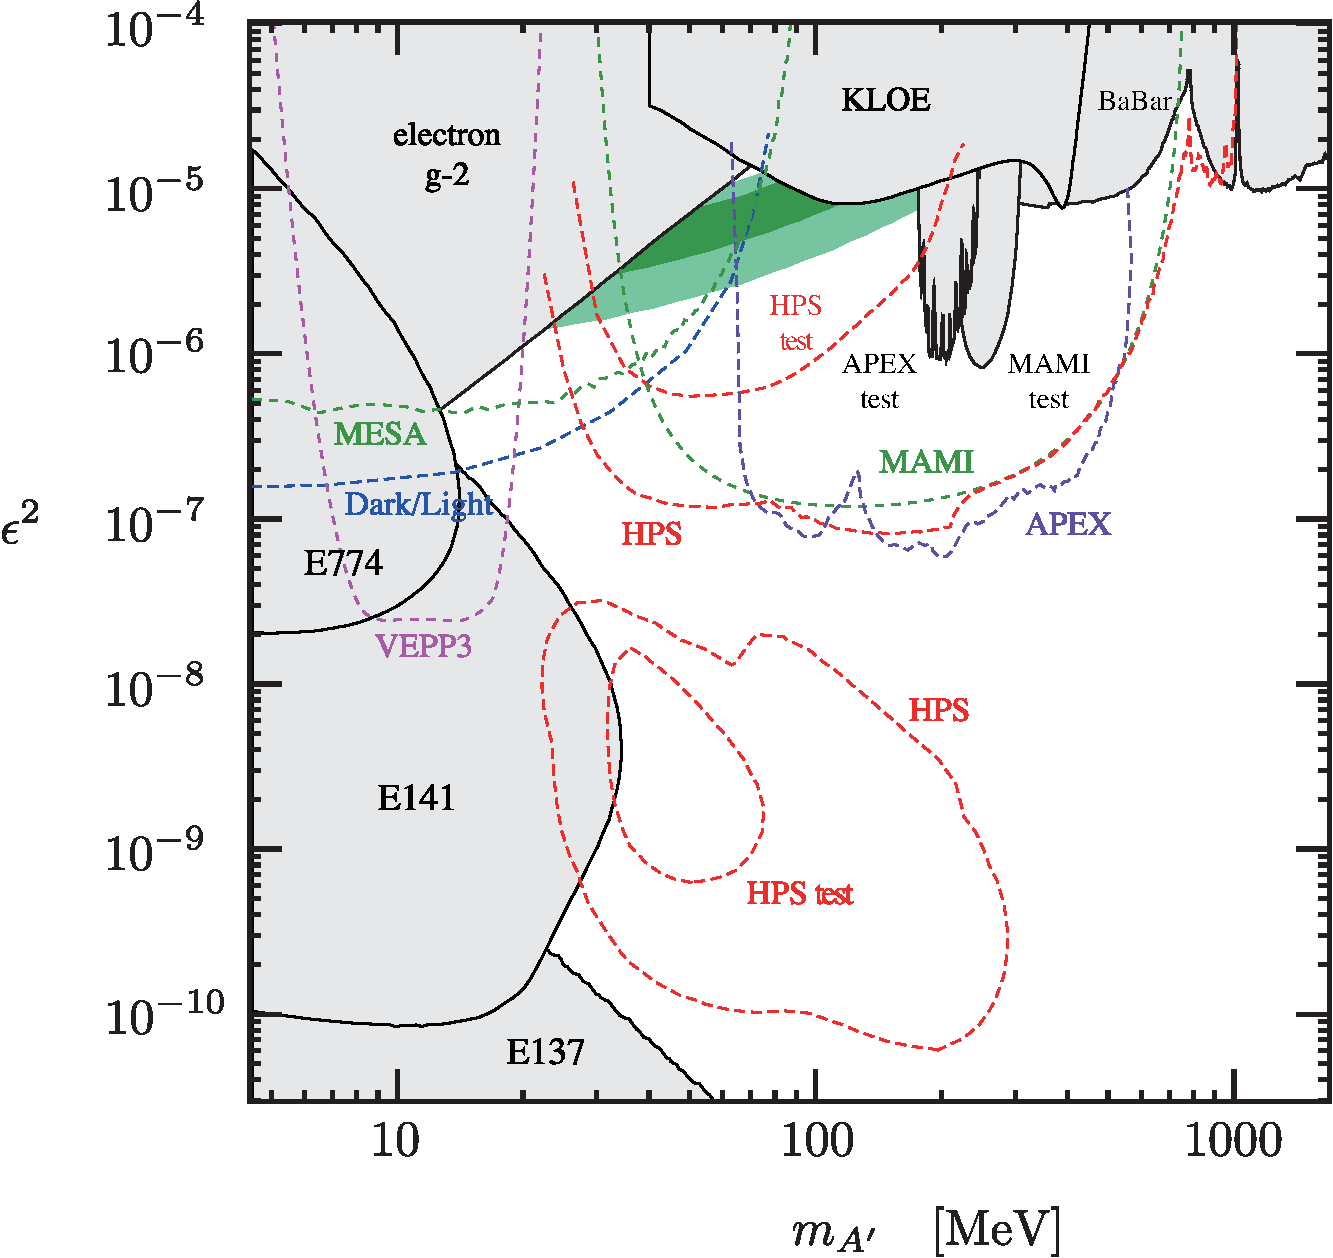
\includegraphics[width=0.8\textwidth]{limit_g-2_electron.pdf} 
\caption{ Existing constraints on heavy photons ($A'$). 
Shown are existing 90\% confidence level limits from the beam dump experiments 
E141, E774, Orsay, and U70~\cite{Bjorken:2009mm,Blumlein:2011mv,Andreas:2012mt,Riordan:1987aw,Bross:1989mp,Davier:1989wz,Konaka:1986cb}, 
the muon anomalous magnetic moment $a_\mu$~\cite{Pospelov:2008zw},  
KLOE~\cite{Collaboration:2011zc}, 
the test run results reported by APEX~\cite{Abrahamyan:2011gv} and MAMI~\cite{Merkel:2011ze}, 
an updated estimate using a BaBar result~\cite{Bjorken:2009mm,Reece:2009un,Aubert:2009cp}, 
%a constraint from supernova cooling~\cite{Bjorken:2009mm} as updated in~\cite{Dent:2012mx}, 
and an updated constraint from the electron anomalous magnetic moment~\cite{endo:g2e,Davoudiasl:2012ig}. 
In the green band, the $A'$ can explain the observed discrepancy between the
calculated and measured muon anomalous magnetic moment~\cite{Pospelov:2008zw} 
at 90\% confidence level.
%Projected sensitivities are shown for the full APEX run~\cite{Essig:2010xa}, 
%DarkLight~\cite{Freytsis:2009bh}, and VEPP-3~\cite{Wojtsekhowski:2009vz}.  
%MAMI has plans (not shown) to probe similar parameter regions as these experiments. 
%Several projected sensitivities are shown for HPS. Solid red shows the 2$\sigma$ limits from the full HPS experiment, assuming 3 months of running time at each of 2.2 GeV(200 nA) and 6.6 GeV (450 nA). The upper region corresponds to a resonance search, the lower to a combined resonance plus vertexing search. Dashed red shows the limits from 1 week of running the HPS Test Run at 2.2 GeV (200 nA). The dashed blue limits corresponds to 1 week of running the Test Run at 1.1 GeV (200 nA).  
%Existing and future $e^+e^-$ colliders like \babar, BELLE, KLOE, Super$B$, BELLE-2, and KLOE-2  can also probe large 
%parts of the parameter space for $\epsilon\gtrsim 10^{-4}-10^{-3}$ (not shown).  
}
\label{fig:hspaw-heavy-A'}
\end{figure*}
%%%%%%%%%%

\subsubsection{Heavy Photons and Dark Matter}
The possible role of heavy photons in the physics of dark matter~\cite{ArkaniHamed:2008qn,Pospelov:2008jd} has provided an urgent impetus to search directly for heavy photons.  Results from two classes of dark matter searches --- ``indirect'' searches for galactic dark matter annihilation and ``direct'' searches for dark matter scattering off nuclei --- have both been interpreted as potential signals of dark matter interacting through a heavy photon.  Both areas have developed considerably in recent years, but not decisively.  Here we briefly summarize the status of dark matter, the case for its interactions with heavy photons,  and pertinent recent developments in both observation and theory.  The motivation to test these theories of dark matter in a controlled laboratory experiment remains strong.    

The concordance model of big bang cosmology --- the Lambda Cold Dark Matter ($\Lambda$CDM) model --- explains all observations of the cosmic microwave background, large-scale structure formation, and supernovae, see 
e.g.~\cite{LambdaCDMData}. This model suggests that Standard Model particles make up only about 5\% of the energy density in the Universe, while ``dark energy'' and ``dark matter'' make up 68\% and 27\%, respectively, of the Universe's energy density. The concordance model does not require dark matter to have any new interactions beyond gravity with Standard Model particles. However, an intriguing theoretical observation, dubbed the ``WIMP miracle'', suggests that dark matter does have new interactions. In particular, if dark matter consists of ~10 GeV to 10 TeV particles interacting via an electroweak-strength force (weakly interacting massive particles or WIMPs), they would automatically have the right relic abundance consistent with the $\Lambda$CDM model.

If dark matter does interact with ordinary matter, such interactions could produce at least two observable consequences: dark matter particles in the Milky Way Galaxy (and other bound astrophysical systems) can annihilate or decay into visible matter, which could be detectable as energetic cosmic rays and/or gamma rays at Earth (indirect detection).  Dark matter passing through Earth can also scatter off nuclear targets, causing the target to recoil.  This recoil is observable in radio-pure detectors with sufficiently low background rates of nuclear recoil (direct detection).  

%Dark matter annihilating into heavy photons offers one explanation for the cosmic-ray electron and positron excesses observed by PAMELA, Fermi, ATIC, and HESS.  
%Such models predict correlated gamma-ray fluxes from other astrophysical systems where dark matter can annihilate (such as the inner galaxy, distant galaxies and clusters) and an imprint in the cosmic microwave background (CMB) from dark matter annihilation in the early Universe.  Since dark matter annihilation into heavy photons was first proposed, limits on gamma-ray fluxes from the above systems have  constrained the parameter space significantly.   However, large theoretical uncertainties  both the rate of dark matter annihilation and the efficiency for gamma-ray production reduce the power of these limits.    
%the gamma-ray flux depends in part on how electrons lose  medium into which electrons are emitted (magnetic field density, density of starlight) electrons  (firstly, because gamma-ray fluxes depend in part on  bounds suffer large (mainly astrophysical) theoretical uncertainties, and their implications for the dark matter models of interest are disputed in the literature.  However, the dark photon mass range that remains viable when these uncertainties are taken into account overlaps considerably with the projected sensitivity of HPS.   

\paragraph{Indirect Detection}The satellites PAMELA \cite{Adriani:2008zr} and Fermi \cite{Ackermann:2010ij}, the balloon-borne detector ATIC \cite{Chang:2008aa}, the ground-based Cherenkov telescope HESS \cite{Aharonian:2008aa,Aharonian:2009ah}, and other experiments have all reported an excess in the cosmic-ray flux of electrons and/or positrons above backgrounds expected from normal astrophysical processes.  
The evidence for this excess has only grown, with new measurements of the cosmic-ray electron flux by PAMELA \cite{Adriani:2011xv} and confirmation by Fermi and AMS-2 of the positron excess \cite{FermiLAT:2011ab,AMS2:2013}.  While further data from AMS-2 may shed more light on the spectrum of these excess cosmic-rays, the origin of these excess positrons and electrons remains unknown.  It may plausibly arise from any of three possibilities: pair creation in nearby pulsars, acceleration in supernova shocks, or dark matter annihilation or decay.

If the excess arises from dark matter annihilation, two features are incompatible with annihilation of ``conventional'' thermal WIMP dark matter charged under the Standard Model weak interactions, but compatible with an alternative explanation, namely that dark matter is charged under a new $U(1)'$ and annihilates into $A'$ pairs, which decay directly into electrons and positrons, and/or into muons that decay into electrons and positrons (see e.g. \cite{ArkaniHamed:2008qn,Pospelov:2008jd,Cirelli:2008pk,Cholis:2008qq,Cholis:2008wq}): 
\begin{itemize}
\item The annihilation cross-section required to explain the electron signal is $50-1000$ times larger than the cross-section favored for the ``WIMP miracle''.   This can be explained if dark matter interacts with an $\mathcal{O}$(GeV)-mass $A'$, which mediates a new moderate range force and enhances the annihilation rate at low velocities (the relative velocity of dark matter in the Galactic Halo, $v\sim 10^{-3} c$, is much lower than in the early universe, and the relative velocity in self-bound dark matter subhalos is lower still).  We refer the reader to \cite{Finkbeiner:2010sm,Slatyer:2011kg} for a recent discussion.
\item The PAMELA satellite did not see any anti-proton excess \cite{Adriani:2008zq}, which implies that, if dark matter annihilation is responsible for the positron/electron signals, it does not produce baryons.  This contradicts expectations for dark matter annihilating through Standard Model interactions, but is expected if dark matter decays into light $A'$, which (for $m_{A'}\lesssim$ GeV) are kinematically unable to decay into protons and anti-protons.
\end{itemize}

We emphasize that these cosmic-ray excesses do not point to a unique region in the $\epsilon-m_{A'}$ parameter space.  
Firstly, the value of $m_{A'}$ determines the branching ratios of the $A'$ (and hence the dark matter, which here is assumed to annihilate to 
the $A'$) to different Standard Model states, including $e^+e^-$, $\mu^+\mu^-$, pions etc.  Since one is trying to match the $e^-$ and 
$e^+$ flux on Earth from dark matter annihilation in the Milky-Way halo to the measured cosmic-ray spectra, the required dark matter 
mass and annihilation cross section is sensitive to the different branching ratios and, hence, $m_{A'}$.   For example, for 
$m_{A'} < 2 m_{\mu}$, the dark matter would almost exclusively annihilate to $e^+e^-$.   However, for $m_{A'} \sim 700$~MeV near the 
$\rho$ or $\omega'$ resonance, the dark matter would annihilate dominantly to pions, decreasing the energy and yield of 
$e^+$ and $e^-$ per annihilation event; this would require a larger dark matter annihilation cross section and larger dark matter mass 
to fit the cosmic-ray spectra.  A large degeneracy thus exists between $m_{A'}$ and the dark matter mass and cross section.  
The degeneracy can be lessened somewhat, but not removed completely, since various other constraints will prefer some regions 
over others (e.g.~$m_{A'}\sim 100$~MeV over 700~MeV).  A set of benchmarks can be found in e.g.~\cite{Finkbeiner:2010sm}, but it will be of interest to cover the whole $m_{A'}$ region as proposed by HPS (even higher masses near 900 MeV would be of interest).  

The second parameter of interest is $\epsilon$.  Unfortunately, $\epsilon$ is almost completely unconstrained by the cosmic-ray data.  The reason is that $\epsilon$ determines the lifetime of the $A'$, but does not affect the dark matter annihilation cross section nor the decay branching ratios of the $A'$ (and hence the dark matter) to Standard Model final states;  and to explain the cosmic-ray anomalies, it is 
irrelevant if the $A'$ decays promptly or only after traveling for thousands of kilometers.  

If dark matter annihilation produces the high-energy $e^+e^-$ excess, correlated gamma-ray fluxes are expected from more distant astrophysical systems where dark matter can annihilate; such fluxes are not expected for the other possible explanations of the cosmic-ray excesses.  Such gamma-ray fluxes have not been seen by satellite or ground-based gamma-ray telescopes, like the the Fermi Gamma-ray Telescope, MAGIC, HESS, or VERITAS.  Bounds on the gamma ray flux from dwarf spheroidals \cite{Ackermann:2011wa}, the outer Milky Way \cite{DiffuseGalactic}, the Galactic Center (e.g. \cite{Papucci:2009gd,Hutsi:2010ai} and references therein), and distant galaxies \cite{Hutsi:2010ai,Zavala:2011tt} and clusters \cite{Huang:2011xr} can thus be used to constrain dark matter interpretations of the Pamela/FERMI excess.  
In a similar spirit, dark matter annihilation in the epoch of atomic recombination would leave an imprint in the cosmic microwave background radiation, which is similarly constrained \cite{CMBrefs}, and the self-interaction of dark matter via $A'$ exchange could affect the shape of galactic halos \cite{Feng:2009hw,Buckley:2009in}.  Each of these systems can be used to constrain models of the PAMELA/Fermi excess, albeit with large theoretical uncertainties.  
%While the present situation (described below) is quite inconclusive, it should be noted that new CMB data expected from Planck will improve sensitivity to dark matter annihilation at the time of recombination by a factor of 10 over WMAP \cite{CMBrefs}.  Thus Planck should either find evidence for dark matter annihilation with a high cross-section (providing further support for dark matter interpretations of the $e^+e^-$ excess), or more robustly constrain the minimal theories.  

The present situation can perhaps be summed up as follows: corroborating evidence for an explanation of the cosmic-ray excesses 
in terms of annihilating dark matter 
\emph{could} have shown up, but have not.  However, the size of the expected corroborating signals is very uncertain, so that the 
present situation is still inconclusive. 
Perhaps the best hope for a more definitive statement on a dark matter origin of the cosmic-ray excesses will arise from new CMB polarization data 
expected from Planck, which will improve sensitivity to dark matter annihilation at the time of recombination by a factor of 10 over WMAP \cite{CMBrefs}.  Planck should either find evidence for dark matter annihilation with a high cross-section (providing further support for dark matter interpretations of the $e^+e^-$ excess), or more robustly constrain the minimal theories.  
We note that the recent release of the Planck data only included the temperature data, and the resulting constraints will be 
only minimally improved in comparison to the previously available data from WMAP9, the Atacama Cosmology Telescope (ACT), and the 
South Pole Telescope (SPT).  A significant improvement is expected next year, when the CMB polarization power spectrum from 
Planck, ACT, and SPT will become available.  

A very important caveat to the above discussion is that we assumed that dark matter \emph{annihilations} to $A'$s are the origin of the excesses.  
Instead, dark matter \emph{decays} to an $A'$ and other light hidden sector particles are also a viable 
possibility~\cite{Essig:2010ye,Ruderman:2009tj}.  
In this case, an $A'$ mass 
below $\sim 1$~GeV is again motivated by the absence of an antiproton signal, but the size of the $e^+/e^-$ signal is set by the 
dark matter decay lifetime, and independent of the $A'$ mass (recall that in the case of dark matter annihilations, the $A'$ mass was an important 
ingredient in determining the size of the Sommerfeld enhancement and, thus, the annihilation cross section).  
Dark matter decays are less constrained than annihilations as a possible origin to the cosmic-ray excesses, as they produce a smaller 
corroborating gamma-ray signal (this signal is now proportional to the dark matter density $\rho$ and not $\rho^2$).  Also, no 
evidence is expected to show up in the CMB data, since the required dark matter lifetime to explain the cosmic-ray excesses is $\sim 10^{26}$~seconds, much larger than the time of the CMB formation ($\sim 10^{13}$~seconds).  

%Accounting for substructure at the level suggested by e.g.~\cite{Kamionkowski:2010mi},  light-$A'$ regions easily avoid constraints from the CMB, galactic center, dwarf galaxies, and dark matter self-interaction (though improved measurements of the CMB by Planck could severely constrain even these scenarios)~\cite{Slatyer:2011kg}.   Constraints on dark matter annihilation in distant galaxies (which would give rise to a diffuse and isotropic gamma-ray signal over the entire sky) are potentially severe even for these light-$A'$ models, but subject to theoretical uncertainties of several orders of magnitude.  In summary, light-$A'$ models of dark matter annihilation are consistent with all other data, but their viability depends on aspects of the dark matter distribution that are not yet reliably understood.

\paragraph{Direct Detection}
 The search for dark-matter-nuclear scattering has also seen considerable developments recently, but remains equally ambiguous.  Four experiments have reported excesses that \emph{may} be attributable to dark matter, although more mundane explanations 
are certainly possible: DAMA/Libra \cite{Bernabei:2010mq}, CoGeNT \cite{Aalseth:2010vx}, which also reported an annual modulation signal \cite{Aalseth:2011wp},  CRESST \cite{Angloher:2011uu}, and CDMS-Silicon \cite{Agnese:2013dwa}. 
If all or a subset of these signals have a dark matter origin,  they are most readily attributed to light dark matter ($\sim 10$ GeV).  
However, results from CDMS-Germanium \cite{CDMS}, XENON10 \cite{Angle:2011th}, and XENON 100 \cite{Aprile:2011hi} appear to disfavor the same parameter regions.  Experimental and detector uncertainties remain large enough that perhaps some model parameter space remains 
moderately consistent with all of these results \cite{Kelso:2011gd,Frandsen:2013cna}.  In fact, a recent re-analysis of the XENON10 constraint in~\cite{Frandsen:2013cna} found a mistake in the original XENON10 publication \cite{Angle:2011th}, which weakens the published limit by a factor of a few.  The situation is very fluid; more data is forthcoming and will shed light on the current situation.
Though the evidence for light dark matter is controversial, it does raise a puzzle: dark matter with such low masses and high couplings cannot easily interact through Standard Model forces (such as $Z$-boson exchange), without being excluded by measurements of the total $Z$ width at LEP. If indeed dark matter is light, then it seems most likely to interact through a new mediator, a possibility that HPS will probe in the case of an $A'$.

We note that heavy inelastic dark matter ($\sim 100-1000$~GeV) interacting with nuclei through $A'$-exchange was a possible explanation for 
these direct detection anomalies a few years ago, and its annihilation to $A'$s could also have explained the cosmic-ray excesses.  However, 
this possibility is now highly constrained by results from XENON100~\cite{Aprile:2011ts} and CRESST~\cite{Angloher:2011uu}.  Light dark matter, 
as mentioned above, is still viable.  In order to have a unified dark matter explanation of the cosmic-ray excesses and direct detection 
anomalies, one would now likely need two components of dark matter, one light and one heavy component.  Theoretical examples of 
such a possibility have been discussed in the literature, see e.g.~\cite{Essig:2010ye}.


\subsubsection{Heavy Photons and Muon $g-2$}

Besides being theoretically natural and having a possible connection to dark matter, an $A'$ could explain the discrepancy between the measured and 
calculated value of the anomalous magnetic moment of the muon $(a_\mu=g-2)$~\cite{Pospelov:2008zw}.  
This long-standing puzzle has several possible resolutions, but among the simplest new physics explanations
is the existence of a new force mediator that couples to muons, like the $A'$.  The contribution to $a_\mu$ of the $A'$ 
is like that of the photon, but suppressed by the mixing parameter $\epsilon^2$ and dependent on the $A'$ mass.  
The green region in Fig.~\ref{fig:hspaw-heavy-A'} is the 2$\sigma$ band in which the $A'$ can 
explain the discrepancy.  This is an intriguing region, which the HPS experiment will probe.  

\subsection{Update on Experimental Status}

The most recent (as of October 2012) comprehensive update summarizing the experimental status of $A'$ searches 
can be found in the presentations and summary talk of the Frascati ``Dark 2012'' workshop~\cite{Dark2012}.
All relevant measurements and constraints, as of this workshop, are included in Fig.~\ref{fig:hspaw-heavy-A'}.
One important change relative to a year ago is that an improved measurement of the Rydberg energy scale 
has allowed previous measurements of $g-2$ of the electron to constrain the allowed parameter space somewhat (in the low $A'$ mass range)
%has slightly reduced the range of allowed parameter space (on the low mass range) for an $A'$ to explain the $g-2$ of the muon 
%discrepancy
~\cite{endo:g2e,Davoudiasl:2012ig}.  
Additionally, searches for $A'$s in rare $\phi$ decays at KLOE and rare $\pi^0$ decays at WASA have slightly reduced 
the allowed parameter space on the high mass range~\cite{rarek}. 
%An ongoing search in the $e^+e^-$ spectrum of data recently gathered by MAMI~\cite{Merkel:2011ze} should also 
%be sensitive to the $A'$ mass range explored by KLOE, but with sensitivity down to roughly $\epsilon\sim 10^{-3}$. 
Finally, improved theoretical calculations and modeling of the experimental acceptance have led to slightly revised constraints on the 
$A'$ parameter space from past beam dump experiments sensitive to $A'$ production and decay to $e^+e^-$ pairs~\cite{andreas}.

\subsection{HPS physics with True Muonium}

Positronium and muonium, bound states of $(e^+ e^-)$ and $(\mu^+ e^-)$ pairs, respectively, have been
produced and studied \cite{Deutsch:1951zza,Friedman:1957mz,Hughes:1960zz}, but True Muonium has not yet been 
detected (see e.g. \cite{Holvik:1986ty,ArteagaRomero:2000yh,Brodsky:2009gx,Bilenky:1969zd,Hughes:1971,Malenfant:1987tm,Karshenboim:1998we,Owen:1972,Jentschura:1997ma,Jentschura:1997tv,Karshenboim:1998am}. 
Together with tauonium $(\tau^+ \tau^-)$ and tau-muonium $(\tau^{\pm} \mu^{\mp})$, True Muonium is among the most
compact pure QED systems. While $(\tau^+ \tau^-)$ and $(\tau^{\pm} \mu^{\mp})$ are difficult to detect since the $\tau$ has a
weak decay that competes with the QED decay, the $\mu$ is very long lived so that the decay of True
Muonium is purely a QED process. 

The detection of True Muonium would be a significant discovery and would constitute a further important test of QED.   
A number of applications of True Muonium measurements have been highlighted in 
\cite{Brodsky:2009gx}, designed to exploit True Muonium as a perturbative laboratory 
for QCD bound state physics. 
These include measuring dissociation cross-sections as a function of energy and lifetimes of the various states. 
More speculatively, the discrepancy between theory and experiment for $g-2$ of the muon~\cite{Bennett:2006fi} and the discrepant measurement of
the charge radius of the proton using muon bound states~\cite{Pohl:2010zza} suggest that further measurements of 
muon properties would be useful to resolve these puzzles. 

%That HPS will be the first experiment capable of detecting True Muonium is straightforward to understand. 
%The triplet True Muonium states $1^3S_1$, $2^3S_1$, and $2^3P_2$ all eventually decay 
%to $e^+e^-$ final states, with lifetimes long enough to leave a detectable displaced vertex.
%In that important respect, triplet True Muonium states behave just like $A'$s. 
%True Muonium production kinematics is a bit different. 
%In HPS, True Muonium will be produced by electron scattering off the high-$Z$ nuclear target. 
%The so-called ``single-photon'' production mechanisms gives rise to True Muonium states with kinematics extremely similar to $A'$s -- HPS will be most 
%sensitive to these. The ``three-photon'' production mechanism, which is typically larger, gives rise to True Muonium with characteristically lower energy. 
 
Studies of the production and dissociation of True Muonium suggest
that the yields in HPS should be sufficient for observation
\cite{Banburski:2012tk}, and are discussed further in section 3. That
HPS is uniquely suited for detecting True Muonium is straightforward
to understand.
The triplet True Muonium states $1^3S_1$, $2^3S_1$, and $2^3P_2$ all
eventually decay
to $e^+e^-$ final states, with lifetimes long enough to leave a
detectable displaced vertex.
In that important respect, triplet True Muonium states behave just like $A'$s.
True Muonium production kinematics is a bit different.
In HPS, True Muonium will be produced by electron scattering off the
high-$Z$ nuclear target.
The so-called ``single-photon'' production mechanisms gives rise to
True Muonium states with kinematics extremely similar to $A'$s -- HPS
will be most
sensitive to these. The ``three-photon'' production mechanism, which
is typically larger, gives rise to True Muonium with
characteristically lower energy. 
 
In addition to primary production mechanisms, there are a variety of secondary mechanisms
that are important in targets thicker than $\sim0.01\%$ radiation lengths.
This was studied in some detail in \cite{Banburski:2012tk}, where it was 
shown that $1^3S_1$ excitations (in the target) are the main source of 
$2^3S_1$ and $2^3P_2$ production.
The $2S$ and $2P$ state are especially long-lived, so this finding
suggests that HPS may first discover these states as they will comprise 
a sizable fraction of the $e^+e^-$ decays with displaced vertex in the range of $\sim 1$ cm to several cm. 
The $1S$ state will be the main component of the decays in the region of  $\sim 1$ cm and below. 

\subsection{HPS Searches for Hidden Sectors}

As highlighted in the Intensity Frontier Workshop report \cite{Hewett:2012ns},
a well-motivated class of beyond the Standard Model scenarios include new particles that interact
indirectly or very weakly with Standard Model matter (hidden sectors), possibly associated with dark matter. 
Low-energy and high-intensity experiments offer an excellent tool for exploring these
possibilities, complementary to the ongoing efforts at high energy colliders. 

HPS is primarily desinged to look for new sub-GeV $A'$s that decay into lepton pairs.
But if an $A'$ is part of a larger hidden sector, as is often assumed in the literature, 
some fraction of the decays could be more intricate.
For example, an $A'$ might decay into hidden sector particles, which in turn may decay back into Standard Model lepton or photons.  
These decays would tyically have displaced vertices and multiple leptons or photons. The phenomenolgofy of a variety of such scenarios 
have been considered in \cite{Strassler:2006im, Essig:2009nc} (and references therein). 
Search strategies to look for more general decays of $A'$s into hidden sector particles are actively being developed within HPS, 
and we comment in more detail on this physics opportunity in Section \ref{sec:hidden_ex}.

%%%%%%%Additional References to Add%%%%%%%%%%%%

